%%%%%%%%%%%%%%%%%%%%%%%%%%%%%%%%%%%%%%%%%
% Beamer Presentation
% LaTeX Template
% Version 1.0 (10/11/12)
%
% This template has been downloaded from:
% http://www.LaTeXTemplates.com
%
% License:
% CC BY-NC-SA 3.0 (http://creativecommons.org/licenses/by-nc-sa/3.0/)
%
%%%%%%%%%%%%%%%%%%%%%%%%%%%%%%%%%%%%%%%%%

%----------------------------------------------------------------------------------------
%	PACKAGES AND THEMES
%----------------------------------------------------------------------------------------

\documentclass[spanish]{beamer}

\mode<presentation> {

% The Beamer class comes with a number of default slide themes
% which change the colors and layouts of slides. Below this is a list
% of all the themes, uncomment each in turn to see what they look like.

%\usetheme{default}
%\usetheme{AnnArbor}
%\usetheme{Antibes}
%\usetheme{Bergen}
%\usetheme{Berkeley}
%\usetheme{Berlin}
%\usetheme{Boadilla}
%\usetheme{CambridgeUS}
%\usetheme{Copenhagen}
%\usetheme{Darmstadt}
%\usetheme{Dresden}
%\usetheme{Frankfurt}
%\usetheme{Goettingen}
%\usetheme{Hannover}
%\usetheme{Ilmenau}
%\usetheme{JuanLesPins}
%\usetheme{Luebeck}
%\usetheme{Madrid}
%\usetheme{Malmoe}
%\usetheme{Marburg}
%\usetheme{Montpellier}
%\usetheme{PaloAlto}
%\usetheme{Pittsburgh}
%\usetheme{Rochester}
%\usetheme{Singapore}
%\usetheme{Szeged}
\usetheme{Warsaw}

% As well as themes, the Beamer class has a number of color themes
% for any slide theme. Uncomment each of these in turn to see how it
% changes the colors of your current slide theme.

%\usecolortheme{albatross}
%\usecolortheme{beaver}
%\usecolortheme{beetle}
%\usecolortheme{crane}
%\usecolortheme{dolphin}
%\usecolortheme{dove}
%\usecolortheme{fly}
%\usecolortheme{lily}
%\usecolortheme{orchid}
%\usecolortheme{rose}
%\usecolortheme{seagull}
%\usecolortheme{seahorse}
%\usecolortheme{whale}
%\usecolortheme{wolverine}

%\setbeamertemplate{footline} % To remove the footer line in all slides uncomment this line
%\setbeamertemplate{footline}[page number] % To replace the footer line in all slides with a simple slide count uncomment this line

%\setbeamertemplate{navigation symbols}{} % To remove the navigation symbols from the bottom of all slides uncomment this line
}

\usepackage{graphicx} % Allows including images
\usepackage{booktabs} % Allows the use of \toprule, \midrule and \bottomrule in tables
\usepackage[utf8]{inputenc} % Para los tildes

\usepackage{babel}
\addto\shorthandsspanish{\spanishdeactivate{~<>}}

\logo{
\includegraphics[height=0.15in]{logo-mina-right.png}}

%----------------------------------------------------------------------------------------
%	TITLE PAGE
%----------------------------------------------------------------------------------------

\title[Robotito]{Programando robots jugando con el entorno}  % The short title appears at the bottom of every slide, the full title is only on the title page
\author[Gonzalo Tejera]{~Gonzalo Tejera\inst{1}}
\institute[FIng::UdelaR]{\inst{1} Instituto de Computación\\
Facultad de Ingeniería\\
Universidad de la República}
\date[MINA 2017]{Grupo MINA, 2017}

%\medskip
%\textit{john@smith.com} % Your email address

\begin{document}

\begin{frame}
\titlepage % Print the title page as the first slide
\end{frame}

\begin{frame}
\frametitle{Contenido} % Table of contents slide, comment this block out to remove it
\tableofcontents % Throughout your presentation, if you choose to use \section{} and \subsection{} commands, these will automatically be printed on this slide as an overview of your presentation
\end{frame}

\section{Introducción}
\begin{frame}
	\frametitle{Motivación}
	\begin{itemize}
		\item Robótica educativa.
		\item Pensamiento computacional.
	\end{itemize}
\end{frame}



\begin{frame}
	\frametitle{Ejemplos de robots}
	\begin{itemize}
		\item Cellulo
		\item KIBO
		\item MOSS
	\end{itemize}
\end{frame}

\begin{frame}
	\frametitle{Objetivos}
	\begin{itemize}
		\item Desarrollar un robot.
		\item Explorar habilidades cognitivas necesarias para utilizarlo.
		\item Evaluar el impacto en las variables cognitivas analizadas.
		\item Evaluar aspectos motivacionales y de cooperación vinculados al juego con robots.
	\end{itemize}
\end{frame}

\begin{frame}
	\frametitle{Contexto}
	\begin{itemize}
		\item CICEA.
		\item Facultad de ingeniería.
	\end{itemize}
\end{frame}

\begin{frame}
	\frametitle{Actividades}
	\begin{itemize}
		\item Relacionamiento con instituciones educativas.
		\item Seminarios con docentes.
		\item Diseño de actividades para la intervención.
		\item Ajustes y definición sobre las herramientas de evaluación.
		\item Capacitación de Equipos Docentes.
		\item Realización del Pre-Test.
		\item Desarrollo de la intervención.
		\item Realización del Post-Test.
		\item Resultados y comunicación.
		\item Sistematización en Protocolo para uso abierto o generalizado.
	\end{itemize}
\end{frame}

\section{Contexto robótico}

\begin{frame}
\frametitle{Proyecto Butiá}
  \begin{columns}[T]
    \begin{column}{.33\textwidth}
    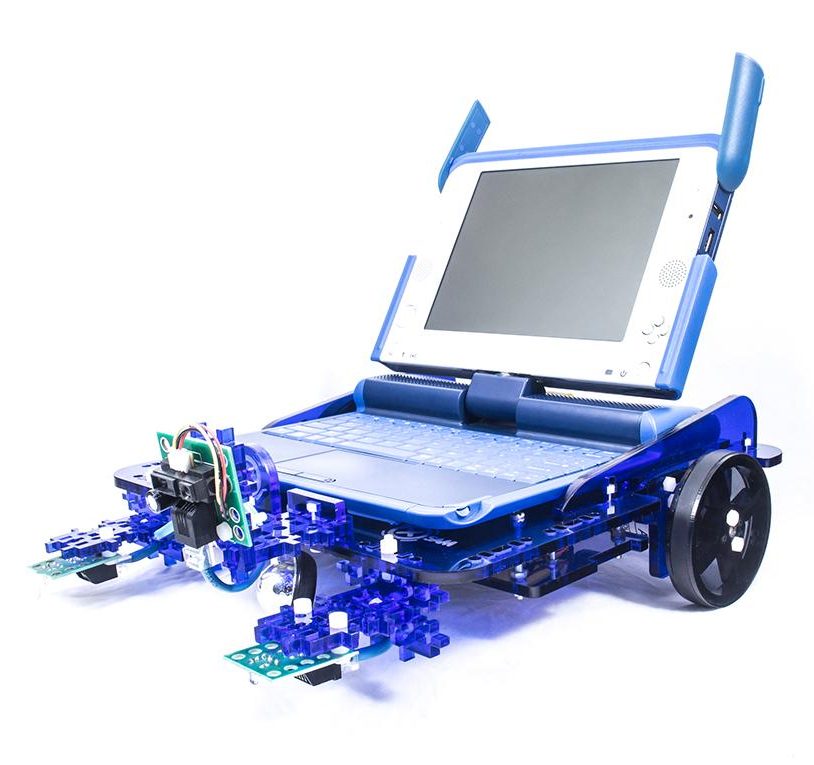
\includegraphics[width=\textwidth]{butia2.png}
    \end{column}
    \begin{column}{.33\textwidth}
    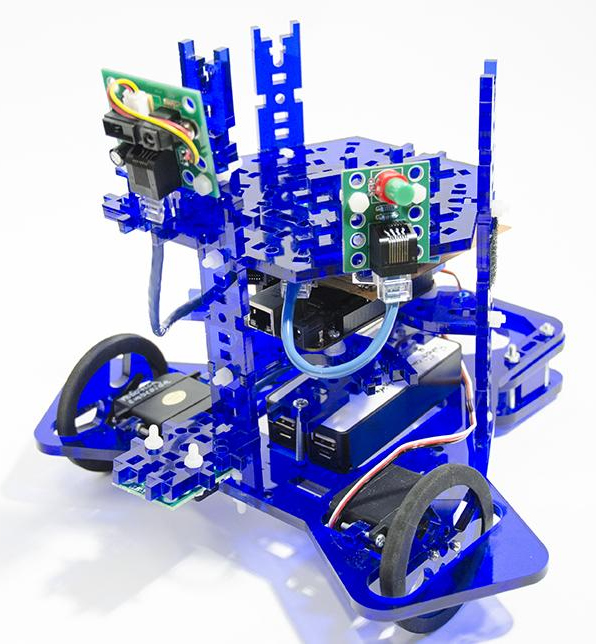
\includegraphics[width=\textwidth]{butia3.png}
    \end{column}
    \begin{column}{.33\textwidth}
    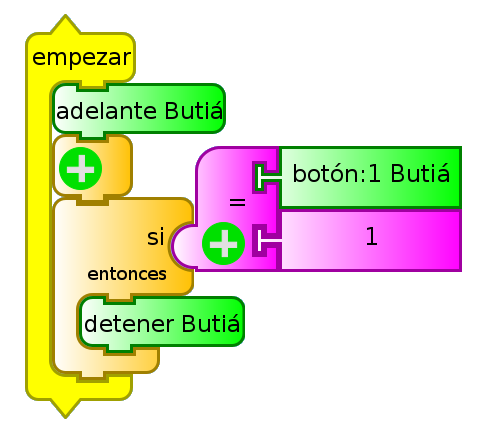
\includegraphics[width=\textwidth]{tortuga.png}
    \end{column}
  \end{columns}
\end{frame}

\begin{frame}
\frametitle{sumo.uy}
	\begin{itemize}
		\item Nueve categorías.
		\item 200 competidores.
		\item 65 equipos.
		\item Presentaciones.
		\item Talleres.
		\item Exposiciones.
	\end{itemize}
\end{frame}

\section{Robotito}

\begin{frame}
	\frametitle{Características}
	\begin{itemize}
		\item Programación a través del ambiente
		\item Acentuar los aspectos corporizados y lúdicos
		\item Mantener las exigencias esenciales de
		\begin{itemize}
			\item descomponer un problema global en componentes simples
			\item la secuenciación adecuada de las operaciones individuales
			\item entre otros aspectos del pensamiento computacional.
		\end{itemize}
		\item Diseñar de una intervención que permita cuantificar los efectos sobre las capacidades que se puedan ver fortalecidas.
	\end{itemize}
\end{frame}

	
\begin{frame}
	\frametitle{Prototipos}
	\begin{itemize}
		\item Faros
		\item Distancia a objetos
		\item Color de los objetos
	\end{itemize}
\end{frame}

\begin{frame}
	\frametitle{Prototipo 1}
	
  \begin{columns}[T]
  	\begin{column}{.5\textwidth}
  		\vspace{1em}
		\begin{itemize}
			\item Omni-direccional
			\item Sensores de distancia
			\item Campos repulsores.
		\end{itemize}
  	\end{column}
  	\begin{column}{.5\textwidth}
		\begin{center}
			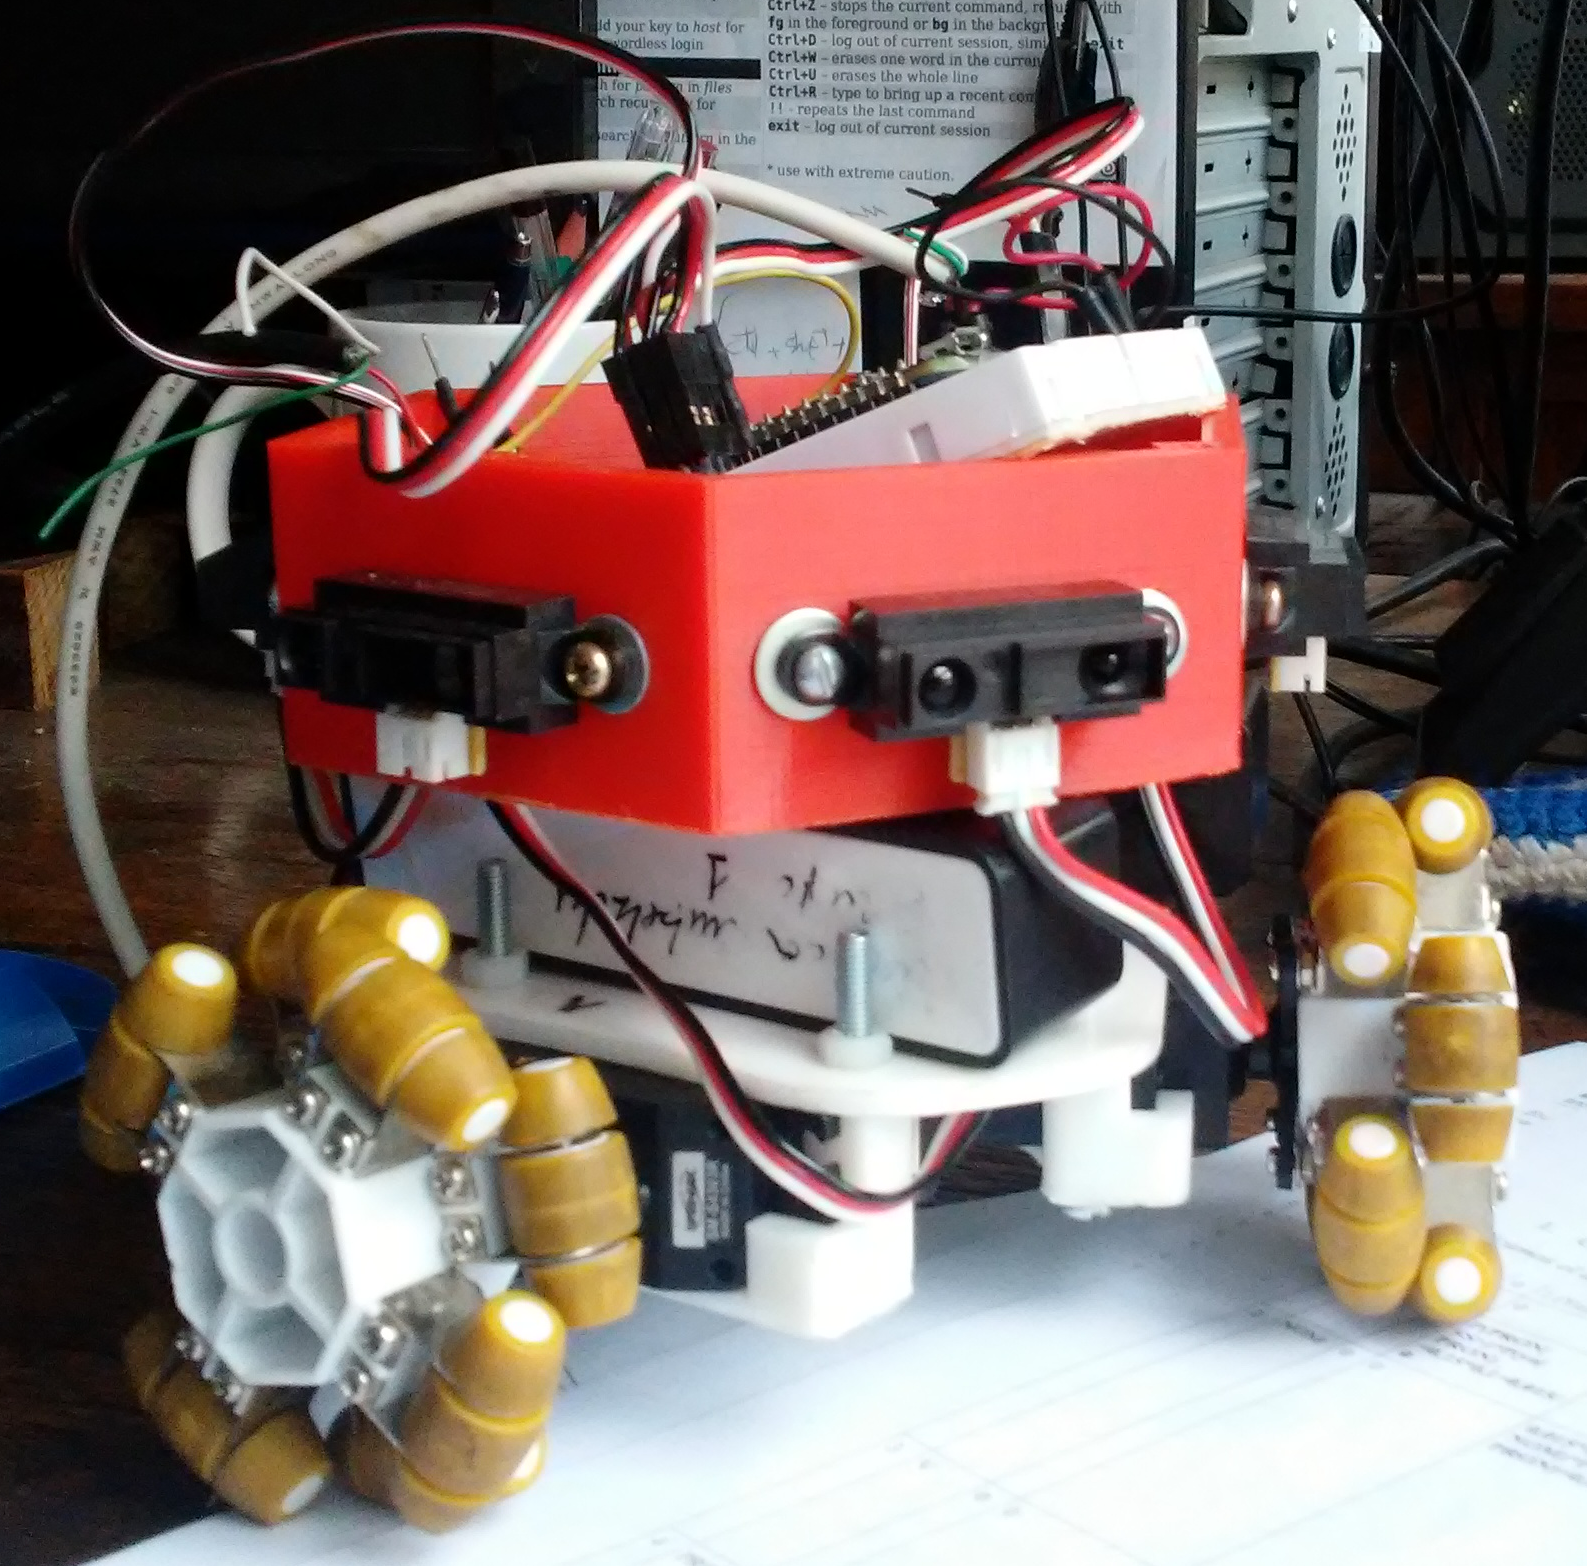
\includegraphics[width=\textwidth]{robotito.png}
		\end{center}
  	\end{column}
  \end{columns}
\end{frame}

\begin{frame}	
\Huge{\centerline{Preguntas}}
\end{frame}

%------------------------------------------------

\begin{frame}
\frametitle{Lecturas Recomendadas}
\footnotesize{

\begin{thebibliography}{99} % Beamer does not support BibTeX so references must be inserted manually as below
\bibitem{butia} Proyecto Butiá.
\newblock Página del proyecto Butiá.
\newblock\emph{www.fing.edu.uy/inco/proyectos/butia}. 2017.

\bibitem{MINA} Grupo MINA.
\newblock Página del grupo MINA.
\newblock\emph{www.fing.edu.uy/inco/grupos/mina}. 2017.

\bibitem{sumo.uy} Sumo robótico.
\newblock Página del evento sumo.uy.
\newblock\emph{sumo.uy}. 2017.

\end{thebibliography}
}
\end{frame}

%----------------------------------------------------------------------------------------

\end{document}
